\documentclass[a4paper,12pt]{article}
\usepackage[english]{babel}
\usepackage{latexsym}
\usepackage{amssymb}
\usepackage{graphicx,epsfig}
%% slashed symbols
\newcommand{\slashed}[1]{\hbox{{$#1$}\llap{$/$}}}


\begin{document}

%%
%% LV exact SUSY massive diagrams
%% LV in the chiral sector
\begin{figure}[h]
 \caption{\label{diag_gauge_massive}
	  Lorentz-violating diagrams in Massive SQED. 
	  Double lines represent chirality-flipping
	  propagators $ \langle \Phi \Phi \rangle $ 
	  and $ \langle \overline{\Phi} \overline{\Phi} \rangle $.
	  Bars denote the $ \overline{\Phi} $ end of propagators.
	  Only $ n_+^\mu $ operator is included in this figure, 
	  the $ n_-^\mu $ operator generates the same
	  set of diagrams. 
	}
\begin{center}
\begin{tabular}{ccc}
 \includegraphics[width=3.2cm,height=3.2cm,keepaspectratio]
		 {diag_gauge_A.ps} &
 \includegraphics[width=3.2cm,height=3.2cm,keepaspectratio]
		 {diag_gauge_B.ps} &
 \includegraphics[width=3.2cm,height=3.2cm,keepaspectratio]
		 {diag_gauge_C.ps} 
\end{tabular}
\begin{tabular}{ccc}
 \includegraphics[width=3.2cm,height=3.2cm,keepaspectratio]
		 {diag_gauge_D.ps} &
 \includegraphics[width=3.2cm,height=3.2cm,keepaspectratio]
		 {diag_gauge_E.ps} &
 \includegraphics[width=3.2cm,height=3.2cm,keepaspectratio]
		 {diag_gauge_F.ps} 
\end{tabular}
\begin{tabular}{ccc}
 \includegraphics[width=3.2cm,height=3.2cm,keepaspectratio]
		 {diag_gauge_massive_A1.ps} &
 \includegraphics[width=3.2cm,height=3.2cm,keepaspectratio]
		 {diag_gauge_massive_A2.ps} &
 \includegraphics[width=3.2cm,height=3.2cm,keepaspectratio]
		 {diag_gauge_massive_A3.ps} 
\end{tabular}
\begin{tabular}{ccc}
 \includegraphics[width=3.2cm,height=3.2cm,keepaspectratio]
		 {diag_gauge_massive_B1.ps} &
 \includegraphics[width=3.2cm,height=3.2cm,keepaspectratio]
		 {diag_gauge_massive_B2.ps} &
 \includegraphics[width=3.2cm,height=3.2cm,keepaspectratio]
		 {diag_gauge_massive_B3.ps} 
\end{tabular}
\begin{tabular}{ccc}
 \includegraphics[width=3.2cm,height=3.2cm,keepaspectratio]
		 {diag_gauge_massive_C1.ps} &
 \includegraphics[width=3.2cm,height=3.2cm,keepaspectratio]
		 {diag_gauge_massive_C2.ps} &
 \includegraphics[width=3.2cm,height=3.2cm,keepaspectratio]
		 {diag_gauge_massive_E1.ps} 
\end{tabular}
\end{center}
\end{figure}


\appendix
\section{Conventions and notations}
\label{app_conventions}

	Our notations for the superfield formalism are based on 
	Wess \& Bagger 
\cite{Wess:1992cp}.
	For conversion between Weyl and Dirac spinors we use the notations
	of 
\cite{Martin:1997ns}.
	Covariant derivatives and hermitean conjugation are taken from
\cite{Gates:1983nr}
	with a proper adaptation.

	The signature of the metric is 
$ (-+++) $.
	All spinor algebra definitions can be found in the canonical treatment
\cite{Wess:1992cp},
	and we list here only some minor conventional departures.

	Unlike in \cite{Wess:1992cp}, we denote the space-time Lorentz
	indices with the letters from the middle of the \emph{greek}
	alphabet:
	$ v_\mu $, $ \sigma_\nu $, $ N^\rho $, etc,
	as it is normally accepted in QFT.
	Spinor indices are taken, also as commonly accepted, from the
	beginning of the greek alphabet:
	$ \theta^\alpha $, $ \epsilon_{\beta\gamma} $, 
	$ \overline{\psi}_{\dot\delta}$.
	Spinor derivatives are designated as
%%
%% spinor derivatives
\[
	\partial_\alpha = \frac{\partial}{\partial\theta^\alpha}\,,
	\qquad
	\partial^\alpha \equiv \epsilon^{\alpha\beta}\partial_\beta
	\,.
\]

	We use a ``slashed'' vector notation in the case where a Lorentz
	vector is contracted with a $ \sigma $-matrix, or a $ \gamma $-matrix:
\begin{equation}
\label{def_slashed}
	\slashed{v} = v^\mu\, \sigma_\mu\;, \qquad
	\overline{\slashed{A}} = A^\mu\, \overline{\sigma}_\mu\;, \qquad
	\slashed{n} = n^\mu \gamma_\mu~~,
\end{equation}
	where the case of $ \sigma $-matrices is used with Weyl spinors, and
	the case of $ \gamma $-matrices is only used with Dirac spinors. 
	There should normally be no confusion as to which kind of spinor is
	meant in a particular expression.
	Note the appearance of the bar upon the slashed vector in
	(\ref{def_slashed}), when it
	is contracted with a $ \overline{\sigma}_\mu $.

	For aesthetical reasons, in cases when two or more close-standing
	factors bear such a bar, we unite them to have one single 
	long bar:
%%
%% Clarification of long bars
\[
	\overline{W W} = \overline{W}_{\dot\alpha}
			 \overline{W}^{\dot\alpha}~,
	\qquad
	\overline{W \sigma_{\mu\nu}\, \slashed{n}}\, W = 
		\overline{W}_{\dot\alpha}\,\, 
		\left(\overline{\sigma}_{\mu\nu}\right)
				^{\dot\alpha}_{~\dot\beta}\,\,
		\overline{\slashed{n}}^{\dot\beta \gamma}\,\,
		W_\gamma~
	~.
\]
	Note, that such a long bar does not symbolize complex conjugation
	of the object beneath it, but instead, indicates that each particular
	factor should be understood as having a bar.

	For switching from Weyl to Dirac spinors we followed the notations of 
\cite{Martin:1997ns}.
	Weyl basis for Dirac spinors is the most appropriate in this case,
	where two Weyl spinors combine into one Dirac spinor:
%% Definition of Dirac spinors
\[
	\Psi = 
		\left (
		\begin{array}{c}
	  		\xi_\alpha \\
			\overline{\chi}^{\dot\alpha}
		\end{array}
		\right )\,,
	\qquad
	\overline{\Psi} = 
		\left (
		\begin{array}{c}
	  		\chi^\alpha \\
			\overline{\xi}_{\dot\alpha}
		\end{array}
		\right )\,,
\]
	and the $ \gamma $-matrices take the form
%%
%% Definition gamma-matrices
\begin{eqnarray*}
	\gamma^\mu = 
			\left ( 
		\begin{array}{cc}
			0                    &    \sigma^\mu \\
                     \overline{\sigma}^\mu   &         0    
		\end{array}
			\right )\,,
	\qquad
	\gamma^5 = 
			\left ( 
		\begin{array}{cc}
			1      &         0  \\
                        0      &        -1    
		\end{array}
			\right )\,.
\end{eqnarray*}
	A bunch of useful conversion formulae can be found
\cite{Martin:1997ns}
	which allow for quick transfer from Weyl-fermionic
	bilinear terms to Dirac-fermionic bilinears:
%%
%% conversion formula between Weyl and Dirac spinors
\begin{equation}
	\begin{array}{ccc}
\renewcommand{\arraystretch}{1.3}
		\begin{array}{l}
		  \overline{\Psi}_1\, \gamma^\mu P_L \Psi_2 =
		    \overline{\xi_1 \sigma_\mu} \xi_2     \\
		  \overline{\Psi}_1\, \gamma^\mu P_R \Psi_2 =
		    \chi_1 \sigma_\mu \overline{\chi}_2
		\end{array}\,,   
\renewcommand{\arraystretch}{1.0}
		&
		~~
		\Psi_1 = \left (
		         \begin{array}{c}
			   \xi_1 \\
			   \overline{\chi}_1
			 \end{array}
			 \right )
		\,,
		&
		~~
		\Psi_2 = \left (
		         \begin{array}{c}
			   \xi_2 \\
			   \overline{\chi}_2
			 \end{array}
			 \right )\,.
	\end{array}
\end{equation}
	The chirality projectors $ P_{L,R} $ are defined as
\cite{Martin:1997ns}:
%%
%% definition of the chirality projectors
\[
	P_L = \frac{ 1 ~+~ \gamma_5 }
                        { 2 }\,,
	\qquad
	P_R = \frac{ 1 ~-~ \gamma_5 }
                        { 2 }~.
\]

	

	Gauge-covariant derivatives are denoted in our paper as
%%
%% definition of covariant derivatives
\renewcommand{\arraystretch}{1.3}
\begin{eqnarray*}
\begin{array}{ll}
        \nabla^+_\alpha = e^{-2eV} D_\alpha e^{2eV}~,
	&
	\qquad
        \overline{\nabla}^+_{\dot{\alpha}} = \overline{D}_{\dot{\alpha}} \\
        \nabla^-_\alpha = D_\alpha~~,
	&
	\qquad
        \overline{\nabla}^-_{\dot{\alpha}} = e^{2eV} \overline{D}_{\dot{\alpha}}
                                    e^{-2eV}~,
\end{array}
\renewcommand{\arraystretch}{1.0}
\end{eqnarray*}
	where the $ + $ or $ - $ superscript relates them to the
	{\it chiral} or {\it antichiral} representation 
\cite{Gates:1983nr}	
	correspondingly
	(in our case, this corresponds to the electron or the positron).
	The symbol $ \nabla^2 $ stands for $ \nabla^\alpha\, \nabla_\alpha $,
	not for $ \nabla^\mu\, \nabla_\mu $, and also
	should not be confused with the d'Alembertian, which we denote
	as:
%% Definition of d'Alembertian
\[
	\Box = \partial^\mu\, \partial_\mu~.
\]

	For the conjugation, we use the notion of 
	\emph{hermitean conjugation} defined
	in 
\cite{Gates:1983nr}.
	When translated into the Wess \& Bagger notations, it implies
\renewcommand{\arraystretch}{1.3}
%%
%% definition of hermitean conjugation
\begin{eqnarray*}
\begin{array}{ll}
% first line
	( \psi_\alpha )^\dagger = \overline{\psi}_{\dot\alpha}~,
	&
	\qquad
	( \psi^\alpha )^\dagger = \overline{\psi}^{\dot\alpha}
	\\
% second line
	\partial_\alpha^\dagger = \overline{\partial}_{\dot\alpha}~,
	&
	\qquad
	\partial_\mu^\dagger = -\, \partial_\mu 
	\\
% third line
	D_\alpha^\dagger = -\, \overline{D}_{\dot\alpha}~,
	&
	\qquad
	( \nabla_\alpha^{\pm} )^\dagger = -\, 
				\overline{\nabla}_{\dot\alpha}^\mp
	\\
% fourth line
	W_\alpha^\dagger = \overline{W}_{\dot\alpha}
\end{array}
\renewcommand{\arraystretch}{1.0}
\end{eqnarray*}
	Its basic principle is that in any expression being
	conjugated {\it all} objects must be put in the reverse order:
%%
%% examples of the conjugation principle
\begin{eqnarray*}
% first line
 	\left( \overline{\Phi}_1 \partial_\mu \Phi_2 \right)^\dagger
	& = & 
	-\, \overline{\Phi}_2 \partial_\mu \Phi_1 \\
% second line
	\left(
	\chi \sigma_\mu \overline{\psi}
	\right)^\dagger
	& = &
	\phantom{-\, }
	\psi \sigma_\mu \overline{\chi} \\
% third line
	\left(
	\chi \sigma_{\mu\nu} \psi 
	\right)^\dagger
	& = &
	-\, \overline{\psi \sigma_{\mu\nu} \chi}~.
\end{eqnarray*}



%%%%%%%%%%%%%%%%%%%%%%%%%%%%%%%%%%%%%%%%%%%%%%%%%%%%%%%%%%%%%%%%
%%%%
%%%      Appendix 
%%%      Vertex Cancellation property
%%%%
%%%%%%%%%%%%%%%%%%%%%%%%%%%%%%%%%%%%%%%%%%%%%%%%%%%%%%%%%%%%%%%%
\section{Cancellation of tadpoles and 
 	the vertex cancellation property}
\label{app_cancellation}

	Cancellation of tadpoles 
%%
%% a simple tadpole with 1 LV insertion
\begin{center}
\includegraphics[width=2.7cm,height=2.7cm,keepaspectratio]{tadpole1.ps}
\end{center}
	can be proved to all orders of Lorentz violation.
	This corresponds to summing all diagrams with arbitrary
	number of LV insertions (\ref{LV_matter})
%%
%% some tadpoles with 1 and 2 LV insertions
\begin{equation}
\label{full_tadpole}
	\begin{minipage}[c]{3.0cm}
	\includegraphics[width=2.7cm]{tadpole1.ps} 
	\end{minipage}
	   +~
	\begin{minipage}[c]{3.0cm}
	\includegraphics[width=2.7cm]{tadpole1d.ps} 
	\end{minipage}
	   +~
	\begin{minipage}[c]{3.0cm}
	\includegraphics[width=2.7cm]{tadpole2.ps} 
	\end{minipage}
	   +~
	   \ldots
	   ~~.
\end{equation}
	In order to show this we evaluate the ``exact'' LV 
	propagator, i.e. a propagator which contains all powers
	of LV:
%%
%% Definition of the full LV propagator
\begin{equation}
\label{def_full_prop}
\begin{minipage}[c]{2.0cm}
\centering
\includegraphics[width=1.7cm]{fullprop.ps} 
\end{minipage}
    \;~\equiv~\;
\begin{minipage}[c]{2.0cm}
\centering
\includegraphics[width=1.7cm]{freeprop.ps} 
\end{minipage}
    ~+~
\begin{minipage}[c]{2.2cm}
\centering
\includegraphics[width=1.9cm]{freeprop1LV.ps} 
\end{minipage}
    ~+~
\begin{minipage}[c]{2.5cm}
\centering
\includegraphics[width=2.2cm]{freeprop2LV.ps} 
\end{minipage}
    ~+~
    \ldots
    ~~.
\end{equation}
	It is straightforward to show that a propagator with $ N $
	LV insertions is
%%
%% The formula for a propagator with N LV vertices
\begin{equation}
\label{N_LV_prop}
	\begin{minipage}[c]{1.7cm}
	\vspace{0.8cm}
	\centering
	\includegraphics[width=1.7cm]{freeprop2LV1.ps}
	\end{minipage}
		\ldots
	\begin{minipage}[c]{1.0cm}
	\vspace{0.78cm}
	\centering
	\includegraphics[width=0.9cm]{freeprop1LV1.ps} 
	\end{minipage}
	~=~ 
	- \frac{i}{p^2}\, \delta^4(\theta_1 - \theta_2)\,
	    (n_e^\mu p_\mu)^N  
	~.
\end{equation}

	Then, the sum in (\ref{def_full_prop}) is a 
	geometric progression: 
%%
%% The formula for the full propagator
\begin{equation}
\label{full_prop}
	\includegraphics[width=1.7cm]{fullprop.ps}
	 \;~=~\;
	- \frac{i}{p^2}\,
		\delta^4 (\theta_1 - \theta_2)\,
		\frac{1}
	           {1 - n^\mu p_\mu}
	~.
\end{equation}
	The full tadpole (\ref{full_tadpole}), in terms of the 
	full propagator, is:
%%
%% The full tadpole
\[
\begin{minipage}[c]{3.0cm}
\centering
\includegraphics[width=2.7cm]{fulltadpole.ps} 
\end{minipage}
	~+~
\begin{minipage}[c]{3.0cm}
\centering
\includegraphics[width=2.7cm]{fulltadpole1.ps} 
\end{minipage}
	~.
\]
	Here the vertices
%% SQED vertex
\begin{minipage}[b]{1.5cm}
\centering
\includegraphics[width=1.2cm]{vertex.ps} 
\vspace{-0.1cm}
\end{minipage}
	and
%% LV SQED vertex
\begin{minipage}[b]{1.5cm}
\centering
\includegraphics[width=1.2cm]{vertex1.ps} 
\vspace{-0.1cm}
\end{minipage}
	exactly sum up into the structure 
$ 1 - n^\mu p_\mu $
	and cancel the denominator in (\ref{full_prop}),
	thus making it to be just a free propagator.
	We are then left with
%%
%% Cancellation at all orders of LV
\begin{equation}
\label{cancellation}
	\begin{minipage}[c]{3.0cm}
	\centering
	\includegraphics[width=2.7cm]{fulltadpole.ps} 
	\end{minipage}
		~+~
	\begin{minipage}[c]{3.0cm}
	\centering
	\includegraphics[width=2.7cm]{fulltadpole1.ps} 
	\end{minipage}
		~~=~~
	\begin{minipage}[c]{3.0cm}
	\centering
	\includegraphics[width=2.7cm]{tadpole.ps} 
	\end{minipage}
	~.
\end{equation}

	That means that Lorentz violation cancels
	{\it to all orders starting from the first}.
	Cancellation of the zeroth order is of course
	a matter of vanishing of the sum of charges 
	in the theory.

	One useful property which is handy for calculations
	can be unscrambled by examining the process of the
	tadpole cancellation (\ref{cancellation}) at the first 
	order of LV:
%%
%% cancellation at the first order of LV
\begin{equation}
\label{cancellation_1LV}
	\begin{minipage}[c]{3.0cm}
	\centering
	\includegraphics[width=2.7cm]{tadpole1.ps} 
	\end{minipage}
	~+~
	\begin{minipage}[c]{3.0cm}
	\centering
	\includegraphics[width=2.9cm]{tadpole1r.ps} 
	\end{minipage}
	~~=~~
	0
	~.
\end{equation}
	This is easy to see from the first order propagator
	(\ref{N_LV_prop}), when $ N $ is put to be equal one.

	In general, 
%%
%% LV vertex
\begin{minipage}[b]{1.5cm}
\centering
\includegraphics[width=1.2cm]{vertex1.ps} 
\vspace{-0.1cm}
\end{minipage}
	corresponds to
%%
%% The expanded superfield expression for the LV vertex
\[
	\frac{1}{2} \overline{n}_e^{\alpha\dot\alpha}
	e\, \overline{\Phi}\,
	\Bigl\{
		\overline{D}_{\dot\alpha} D_\alpha ( V )
		- 
		2 i V \slashed{\partial}_{\alpha\dot\alpha}
	\Bigr\}\,
	 \Phi
	~.
\] 
	Thus, 
%% propagator with 1 LV insertion
\begin{minipage}[b]{1.7cm}
\centering
\includegraphics[width=1.4cm]{freeprop1LV.ps} 
\vspace{-0.06cm}
\end{minipage}
	cancels the second part
	(the term with $ \slashed{\partial}_{\alpha\dot\alpha}$)
	of 
%%
%% LV vertex
\begin{minipage}[b]{1.5cm}
\centering
\includegraphics[width=1.2cm]{vertex1.ps} 
\vspace{-0.1cm}
\end{minipage}
	(in the case of the tadpole (\ref{cancellation_1LV}) 
	this lead to a total 
	cancellation,
	because the 
	$ \overline{D}_{\dot\alpha} D_\alpha V $
	part obviously turns into a total derivative after evaluating
	the first diagram in (\ref{cancellation_1LV})).
	This can significantly decrease the amount of calculations
	by cancelling some parts of (usually different) diagrams.

	This ``vertex cancellation'' property can be extensively
	exploited in loop calculations.

\end{document}
